% Construction : arbre à deux niveaux, racine en (0, 1.5).
%   Niveau 1 : A en (2, 2.6) de probabilité 0,3 ; Ā en (2, 0.4) de probabilité 0,7.
%   Niveau 2 sous A : B en (4.4, 3.2) de probabilité 0,8 ; B̄ en (4.4, 2).
%   La branche AB pèse 0,3 × 0,8 = 0,24.
% SVG : x = 20 + 48x, y = 150 - 42y.
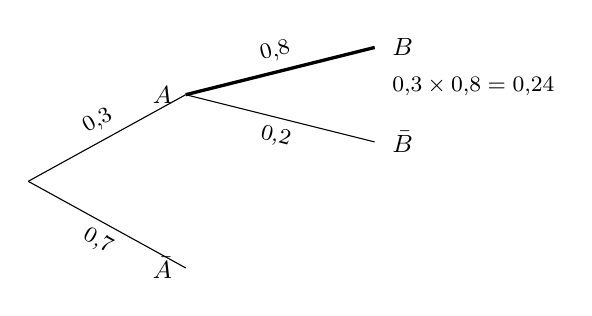
\begin{tikzpicture}[scale=1, >=stealth, every node/.style={font=\small}]
  \draw (0,1.5) -- node[above, sloped, font=\footnotesize] {$0{,}3$} (2,2.6);
  \draw (0,1.5) -- node[below, sloped, font=\footnotesize] {$0{,}7$} (2,0.4);
  \draw[very thick] (2,2.6) -- node[above, sloped, font=\footnotesize] {$0{,}8$} (4.4,3.2);
  \draw (2,2.6) -- node[below, sloped, font=\footnotesize] {$0{,}2$} (4.4,2);
  \node[left] at (1.95,2.6) {$A$};
  \node[left] at (1.95,0.4) {$\bar A$};
  \node[right] at (4.5,3.2) {$B$}; \node[right] at (4.5,2) {$\bar B$};
  \node[right, font=\footnotesize] at (4.5,2.7) {$0{,}3 \times 0{,}8 = 0{,}24$};
\end{tikzpicture}
